\section{Results}
For country-product bi-partite networks,  Caldarelli et al. \cite{caldarelli2012network} found that the ranking of countries correlates reasonably well with their ranking in terms of GDP, after calibration of $\alpha$ and $\beta$ (Pearson correlation $\approx 0.4$ for $\alpha \approx 1.1$ and $\beta \approx 0.8$). Similarly, we studied the correlations of the editors/articles ranking model with grand-truth exogenous values. We studied how these correlations evolve as more edits are contributed to a category of Wikipedia articles. Finally, we investigated the values of calibrated $\alpha$ and $\beta$ in the context of Wikipedia open collaboration.

Figure \ref{fig:rhotime} shows the evolution of the rank correlation (Spearman $\rho$) between $\mathbf{w}^*_e$ and $\mathbf{v}^*_e$, and $\mathbf{w}^*_a$ and $\mathbf{v}_a$ respectively, as a function of time for each of the ten categories ($\alpha$ and $\beta$ are calibrated for each category and each snapshot so that maximum correlation is found). The maximum rank correlation is obtained by numerical optimization {\bf [please describe shortly the method employed]}. The correlations are generally quite high ( $ 0.46 < \rho_e < 0.75$ with $\langle \rho_e\rangle = 0.64$ for editors and $0.57 < \rho_a < 0.91$ with $\langle \rho_a\rangle = 0.72$ ). $\rho_{a}$  is stable over time, which means that the quality of articles can be pretty well captured early on by the model. However, $\rho_e$ exhibits a convex increase over time, suggesting that it takes time (i.e., lots of edits) to capture well the expertise of editors.

{\bf [is there a unique set of $\alpha$ and $\beta$ for $\mathbf{w}^*_a$ and $\mathbf{w}^*_e$ ? Or do you calibrate $\alpha$ and $\beta$ for  $\mathbf{w}^*_a$ and then  $\mathbf{w}^*_e$ ?]}

\begin{figure}[!t]
\centering
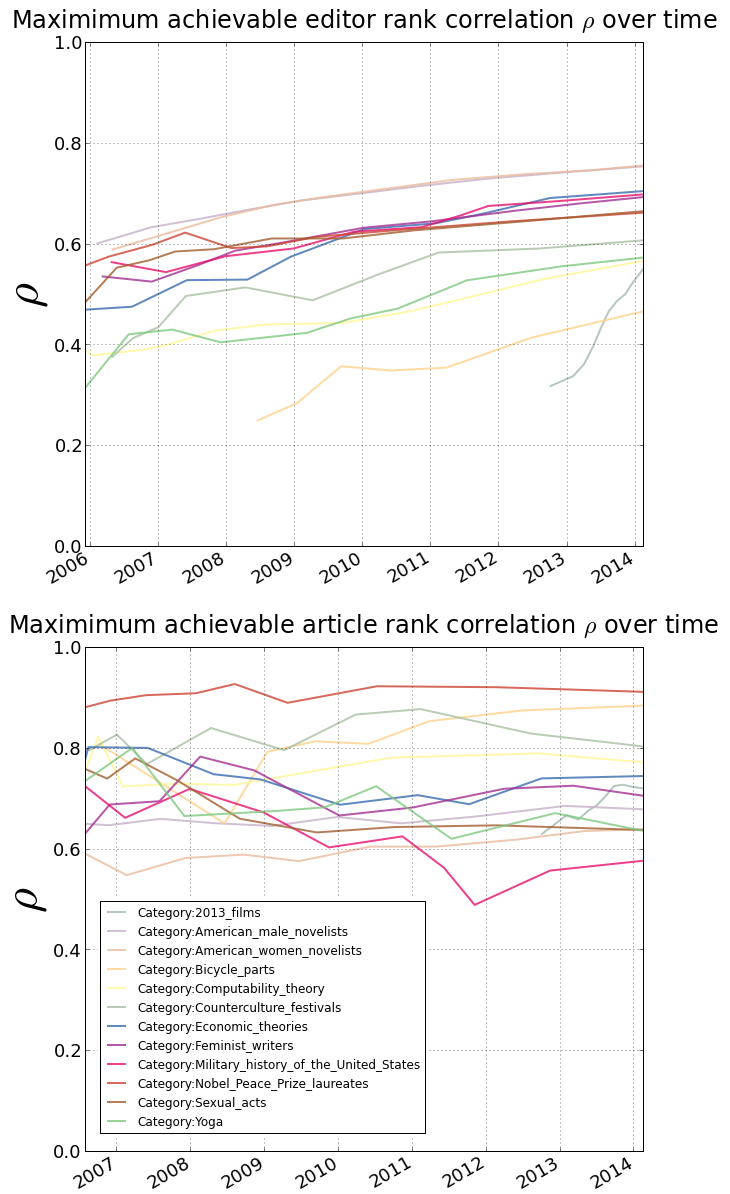
\includegraphics[width=0.9\columnwidth]{Figures/rho_combined.png}.
\caption{Evolution of Spearman $\rho$ rank correlations between the ranking obtained from the calibrated model and the grand-truth values for each category and for editors (upper panel)  and articles (lower panel). The correlations are generally quite high : $ 0.46 < \rho_e < 0.75$ with $\langle \rho_e\rangle = 0.64$ for editors and $0.57 < \rho_a < 0.91$ with $\langle \rho_a\rangle = 0.72$. $\rho_{a}$  is stable over time, which means that the quality of articles can be pretty well captured early on by the model. However, $\rho_e$ exhibits a convex increase over time, suggesting that it takes time (i.e., lots of edits) to capture well the expertise of editors.{\it [please add a label for the x-axis (i.e., Time [years]) and change $\rho$ into $\rho_e$ and $\rho_a$ respectively. You can remove the titles above the  plots]}}
\label{fig:rhotime}
\end{figure}

We now turn to the values of $\alpha$ and $\beta$ for which best correlation is achieved.  Figure \ref{fig:landscape} shows typical landscapes of correlation as a function of $\alpha$ and $\beta$ for editors and articles. It appears that there is no single value of $\alpha$ and $\beta$ for best correlation, but rather some areas (showed by the contour line on Figure \ref{fig:landscape} as the 90th percentile of the rank correlation). The contour line exhibits a linear function between $\alpha$ and $\beta$. For articles, the relationship is typically of the type $\alpha = - b \beta + 1$ for $\beta >0$ with $b$ varying for each category. {\bf [it would make sense to actually evaluate $b$, for instance by making regression of all points above the 90th percentile]} For editors, the relationship is $\alpha = 0$ for $\beta < ??$ {\bf [complete the value once the related plot has been added]}. 

%For editors, maximum $\rho$ always occurs strictly within a radius of 0.01 around the origin on the  $\alpha$-$\beta$ plane. The $(0,0)$ solution is significant in that it represents unbiased arithmetic averages.

%For articles, the solutions have 2-dimensional unbounded triangular solution space. For instance in Category:Economic Theories we find a typical solution space\ref{fig:landscape} . This solution space indicates that the behaviour displayed by the  landscape is a spectrum of possibilities. One one extreme that either $\alpha$ is positive but small, in which case $\beta$ is bounded tightly, which means that fitter editors are producing more obscure articles. Or that $\alpha$ is negative and that $\beta$ is less bounded. This indicates that $\alpha$ is dominating, as is the case in \eqref{eqsim}, and that less fit editors are contributing more, and the ubiquity of their contributions is relatively unimportant. Between categories variations in triangular solution space are rotations around the origin. In our particular example we also find that this solution space is rotated towards the positive $\beta$ axis. So even as the trade triangle occurs, its favours positive $\beta$. Interpreted means that editors who edit relatively more obscure articles are important to success of articles in Category Economic Theories. We do not encounter any rotation in any category that would be large enough to be equivalent to a reflection across the $\alpha = \pm \beta$ axes.

\begin{figure}[!t]
\centering
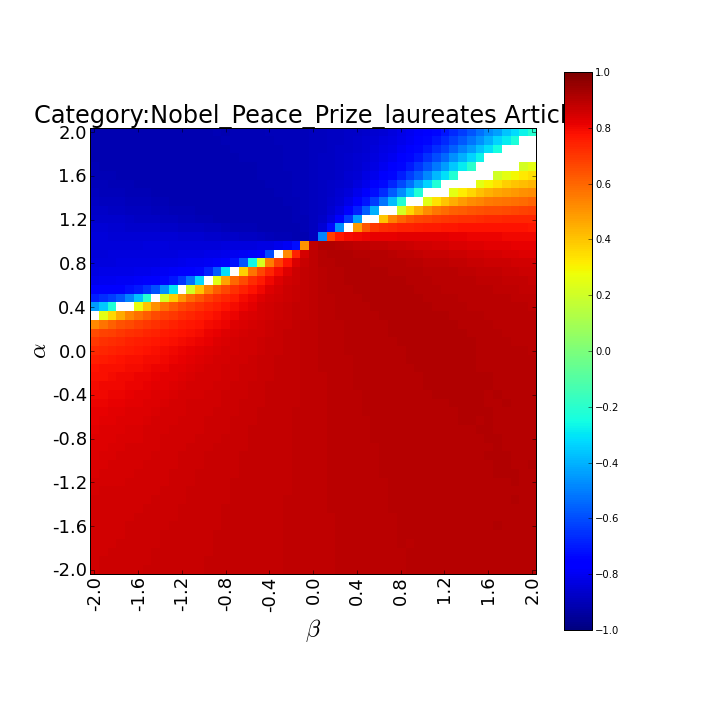
\includegraphics[width=0.9\columnwidth]{Figures/landscape_nobel.png}.
\caption{Typical landscape of maximum correlation as a function of $\alpha$ and $\beta$ for editors (upper panel) and articles (lower panel). The contour line shows the 90th percentile of the rank correlation over the landscape. It typically displays a linear function between $\alpha$ and $\beta$. For articles, the relationship is typically of the type $\alpha = - b \beta + 1$ for $\beta >0$ or $\alpha = b \beta + 1$ for $\beta < 0$ with $b>0$ varying for each category. For editors, the relationship is $\alpha = 0$ for $\beta < ??$. {\it please add the corresponding figure for editors.  that would be great if you could make the labels ($\alpha$ and $\beta$) WAY bigger. You can also get remove the title. The cherry on the cake would be to have the color bar equal or smaller than the vertical dimension of the landscape.}}
\label{fig:landscape}
\end{figure}



%To understand the results, we must have a firm grasp on what $\alpha$ and $\beta$ mean. They are more easily understood by roughly rewriting $\mathbf{w^*}$ as:
%\begin{equation}
%\begin{cases}
%w^{*}_{e} \sim k^{1-\beta}_{e} \langle k_{a}^{-\alpha}\rangle_e \\
%w^{*}_{a} \sim k^{1-\alpha}_{a} \langle k_{e}^{-\beta}\rangle_a
%\end{cases} \label{eqsim}
%\end{equation}
%
%Here we can see the similarity of $w^*$ is related to the product of two expression. Values of $\alpha$ and $\beta$ can make the one of the product close to one or and so the other parameter may dominate.



%$\alpha$ is a measure of how important it is for quality that many users edit, with lower alpha, we have a more collaborative category, where edits are more equal and egalitarean. With alpha high, the category is more rewarding users that operate more individualistically. Beta is inversely related to alpha so the same can be said but the directions of the arguments reversed. This means we can talk of the characteristic of a category, compared to one another and compared over time. 




